\documentclass[a4paper,10pt]{article}

\usepackage[margin=1.2cm]{geometry}
\usepackage{ucs}
\usepackage[utf8]{inputenc}
\usepackage{amsmath}
\usepackage{caption}
\usepackage{subcaption}
\usepackage{graphicx}
% \usepackage{subfigure}
\usepackage{xcolor}
\usepackage[english]{babel}
\usepackage{fontenc}
\usepackage{graphicx}
% \usepackage{mathtools}
\usepackage{siunitx}
\setlength\parindent{0pt}
% \usepackage{psbox}
% \usepackage{auto-pst-pdf}
\usepackage{tikz}
\usetikzlibrary{arrows.meta}

\usepackage{hyperref}

\author{Ömer Faruk Birgül}
% \title{Homework 5}
\title{Midterm}
\date{\today}

\begin{document}
\maketitle
\section*{Q1}
\subsection*{a)}
\begin{figure}[ht!]
 \centering
 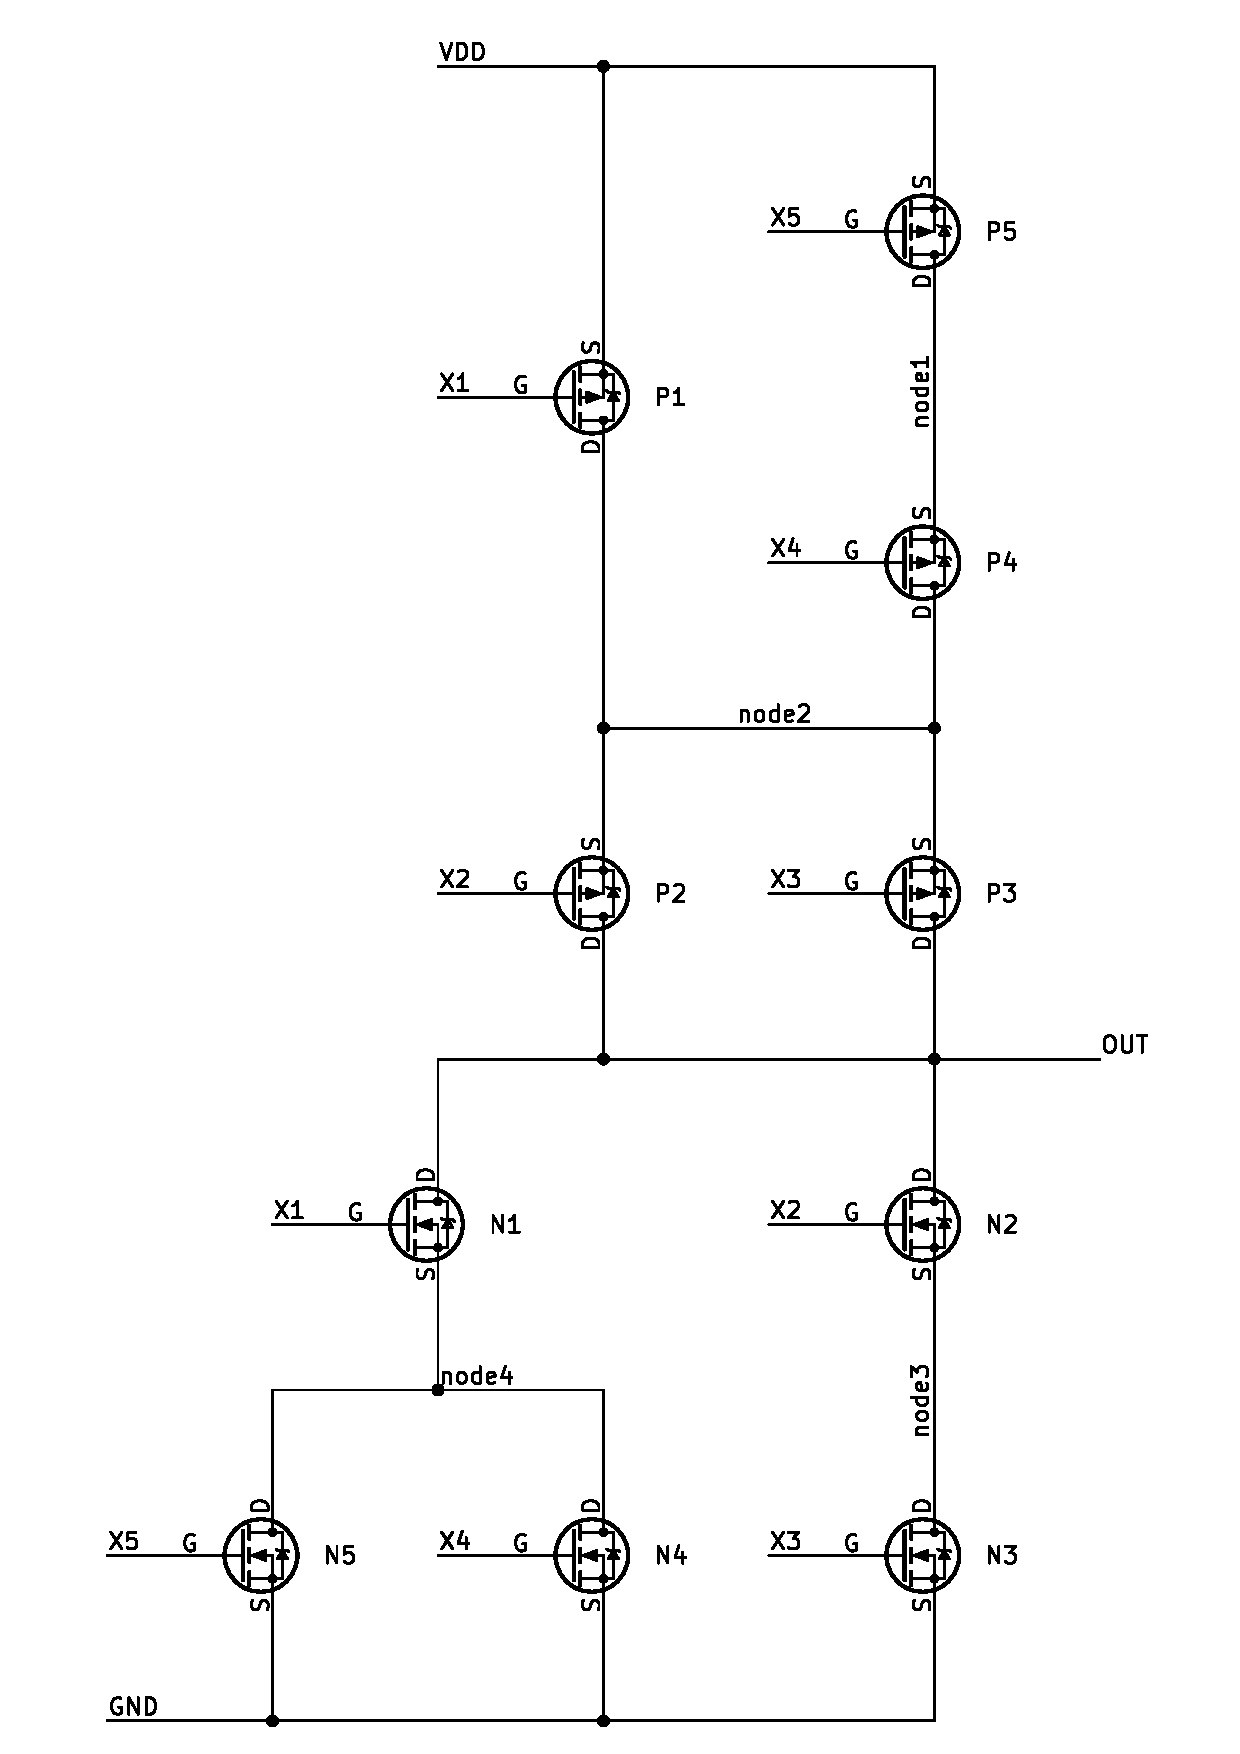
\includegraphics[width=0.7\textwidth]{output.pdf}
 \caption{Schematic of the five input function.}
 \label{fig:sch}
\end{figure}

\newpage
\subsection*{b)}
Output function is $\overline{[(X4+X5).X1+X2.X3]}$

\subsection*{c)}
Nodes are name in the \autoref{fig:sch}.
\begin{verbatim}
MP1 node2 X1 VDD VDD CMOSP W=0.5u L=0.2u
MP2 OUT X2 node2 VDD CMOSP W=0.5u L=0.2u
MP3 OUT X3 node2 VDD CMOSP W=0.5u L=0.2u
MP4 node2 X4 node1 VDD CMOSP W=0.5u L=0.2u
MP5 node1 X5 VDD VDD CMOSP W=0.5u L=0.2u

MN1 OUT X1 node4 0 CMOSN W=0.5u L=0.2u
MN2 OUT X2 node3 0 CMOSN W=0.5u L=0.2u
MN3 node3 X3 0 0 CMOSN W=0.5u L=0.2u
MN4 node4 X4 0 0 CMOSN W=0.5u L=0.2u
MN5 node4 X5 0 0 CMOSN W=0.5u L=0.2u
\end{verbatim}


\newpage
\section*{Q2}
Before starting calculations, I determine all necessary values in \autoref{eq:all_values}, units are given in square brackets. $C_L$, $W_{N(1)}$, $J_{N(max)}$, $J_{P(max)}$, and $L_{min}$ given in the tech file. $CGSO$ is a value from mosfet model. $C_{OX}$ can be calculated usign $\frac{\epsilon_{ox}}{t_{ox}}$ where $\epsilon_{ox}$ is approximately $3.453\text{e-}13[F/cm^2]$, and $t_{ox}$ is from the mosfet model.
\begin{equation}\label{eq:all_values}
\begin{split}
 C_L & = 5.00\text{e-}12[F] \\
 J_{N(max)} & = 508[A/m] \\
 J_{P(max)} & = 224[A/m] \\
 L_{min} & = 2.00\text{e-}7[m] \\
 C_{OX} & = 8.41\text{e-}3[F/m^2] \\
 CGSO & = 7.19\text{e-}10[F/m] \\
 W_{N(1)} & = 5.00\text{e-}7[m]
\end{split}
\end{equation}

\subsection*{Calculation of chain number}
Since n is given as 3, I will use it as 3.

\subsection*{Calculation of tapering factor}
Then I need to calculate $m$ which is calculated by \autoref{eq:formula_2}.
\begin{equation}\label{eq:formula_2}
 n= \left[ \frac{C_L}{\left(1+\sqrt{\frac{J_{N(max)}} {J_{P(max)}}}\right)\cdot(L_{min}.C_{OX}+2\cdot CGSO)\cdot W_{N(1)}}\right]^{\frac{1}{n}}
\end{equation}

And when I put the values to formula:
\[
 n=\left[ \frac{1.00\text{e-}12[F]}{\left(1+\sqrt{\frac{508[A/m]}{224[A/m]}}\right)\cdot(2.00\text{e-}7[m]\cdot8.41\text{e-}3[F/m^2]+2\cdot7.19\text{e-}10[F/m])\cdot5.00\text{e-}7[m]}\right]^{\frac{1}{3}}
\]

And results is $10.85487625$. So $m\approx 10.85$.

\subsection*{a)}
\begin{center}
\begin{tabular}{|l|l|l|}\hline
Inverter & Wn & Wp\\\hline
1 & 500n & 750n\\\hline
2 & 5425n & 8137n\\\hline
3 & 58861n & 88291n\\\hline
\end{tabular}
\end{center}

\subsection*{b)}
I need to calculate $\mathcal{L}$ which is calculated by \autoref{eq:formula_3}.
\begin{equation}\label{eq:formula_3}
\mathcal{L} = \frac{1}{4}\cdot \left(\frac{1}{\sqrt{J_{N(max)}}} + \frac{1}{\sqrt{J_{P(max)}}}  \right)^2 \cdot (L_{min}\cdot C_{OX} +2\cdot CSGO)\cdot V_{DD}\cdot m \cdot n
\end{equation}
And when I put the values to formula:
\[
\mathcal{L} = \frac{1}{4}\cdot \left(\frac{1}{\sqrt{508[A/m]}} + \frac{1}{\sqrt{224[A/m]}}  \right)^2 \cdot (2.00\text{e-}7[m]\cdot 8.41\text{e-}3[F/m^2] +2\cdot 7.19\text{e-}10[F/m])\cdot 1.8[V]\cdot 10.85 \cdot 3
\]

And results is $5.64931\text{e-}10$. So $\mathcal{L}\approx 564 ps$\\

\subsection*{c)}

\newpage
\section*{Q3}
\subsection*{a)}
Let's write $t_{PLH}$ $t_{PHL}$ for inverter, 3 input NAND and 3 input NOR gates in general form.\\

Assume that $R_n=R$ and $R_p=2R$ beacuse we are using minimum dimensions.\\

Assume that $C_{load}=C$.\\

N is 3 for NAND and NOR.


\subsubsection*{Delay of Inverter}
\begin{align*}
t_{PLH}&\approx 0,7.R_p. C_{load} = 0,7.2R.C &= 1,4RC\\
t_{PHL}&\approx 0,7.R_n. C_{load} = 0,7.R.C &= 0,7RC\\
t_{PD} &= \frac{t_{PLH}+t_{PHL}}{2} = \frac{1,4RC+0,7RC}{2} &= 1,05RC
\end{align*}
\subsubsection*{Delay of NAND}
\begin{align*}
t_{PLH}&\approx 0,7.\frac{R_p}{N}. C_{load} = 0,7.\frac{2R}{3}.C &\approx 0,47RC \\
t_{PHL}&\approx 0,7.N.R_n. C_{load} = 0,7.3.R.C &= 2,1RC\\
t_{PD} &= \frac{t_{PLH}+t_{PHL}}{2} = \frac{0,47RC+2,1RC}{2} &= 1,285RC
\end{align*}
\subsubsection*{Delay of NOR}
\begin{align*}
 t_{PLH}&\approx 0,7.N.R_p. C_{load} = 0,7.3.2R.C &= 4,2RC\\
 t_{PHL}&\approx 0,7.\frac{R_n}{N}. C_{load} = 0,7.frac{R}{3}.C &\approx 0,23RC\\
 t_{PD} &= \frac{t_{PLH}+t_{PHL}}{2} = \frac{4,2RC+0,23RC}{2} &= 2,215RC
\end{align*}

\subsubsection*{Delay of NOR + Inverter}
\begin{align*}
t_{PD}= 2,215RC + 1,05RC = 3,265RC
\end{align*}
\subsubsection*{Delay of Inverters + NAND}
\begin{align*}
t_{PD}= 1,05RC + 1,285RC = 2,335RC
\end{align*}

\subsection*{b)}

\end{document}






